% !TEX program = xelatex    
\documentclass[letterpaper]{article}

\newif\ifaaai
\IfFileExists{aaai2026.sty}{\aaaitrue}{\aaaifalse}
\ifaaai
    \usepackage[submission]{aaai2026}
\else
    \usepackage[letterpaper,margin=0.75in]{geometry}
\fi

\usepackage[UTF8]{ctex}
\usepackage{amsmath,amssymb}
\usepackage{booktabs}
\usepackage{enumitem}
\usepackage{float}
\usepackage{graphicx}
\usepackage{multirow}
\usepackage{placeins}
\usepackage{algorithm}
\usepackage{algpseudocode}
\usepackage{array}
\usepackage{pgfplots}
\pgfplotsset{compat=1.18}
\floatname{algorithm}{算法}
\definecolor{paletteRed}{RGB}{141,47,37}
\definecolor{palettePurple}{RGB}{78,25,69}
\definecolor{paletteTan}{RGB}{203,148,117}
\definecolor{paletteGreen}{RGB}{140,191,135}
\definecolor{paletteBlue}{RGB}{62,96,141}
\definecolor{paletteGray}{RGB}{144,146,145}

\ifaaai\else
    \usepackage{hyperref}
    \hypersetup{
        colorlinks=true,
        linkcolor=blue,
        citecolor=blue,
        urlcolor=blue
    }
\fi

\title{面向 MoE-SwiGLU 模型的路由感知 Wanda 剪枝}
\author{Anonymous Submission}
\ifaaai
\affiliations{
    Paper under double-blind review
}
\fi

\begin{document}
\maketitle
\ifaaai\else\twocolumn\fi

\begin{abstract}
Wanda 通过权重幅值与输入激活尺度的乘积构造剪枝分数，是一种简单有效的后训练非结构化剪枝方法。
本文关注 MoE expert 权重内部的非结构化稀疏化，而不是删除整个 expert 或改变 MoE 拓扑。
然而，在混合专家模型（Mixture-of-Experts, MoE）中，普通 Wanda 分数并不能充分描述 expert 被路由器暴露的程度，也没有显式刻画 SwiGLU expert 内部 gate/up/down 三个投影之间的局部误差传播关系。
我们从 MoE 层输出扰动出发，推导出一组适用于 MoE-SwiGLU expert 的路由感知 Wanda 分数。
该方法将 expert 的路由概率、路由强度、SwiGLU 非线性局部斜率以及 down projection 的输出放大效应同时纳入剪枝准则。
在实现上，我们进一步引入 dense-softmax 路由统计、routing-power 调制，以及基于 router trace 的 expert 聚类剪枝，以缓解高稀疏率下普通 Wanda 的性能坍缩。
为了公平比较，我们在 MoE 模型上复现普通 Wanda 作为基线，并在相同校准、稀疏率和评测协议下比较其与 MoE-Wanda 的 perplexity 和 zero-shot accuracy。
实验结果表明，MoE-Wanda 在 Qwen1.5-MoE-A2.7B 和 DeepSeek-V2-Lite 上能够在多个非结构化稀疏率下取得更稳定的性能。
\end{abstract}

\section{Introduction}

大语言模型的能力提升通常伴随着参数规模、显存占用和推理成本的持续增长。
Mixture-of-Experts (MoE) 通过条件计算缓解了这一矛盾：模型包含大量 expert 参数，但每个 token 只激活其中一小部分 expert，从而在增加模型容量的同时控制单次前向计算量。
从早期 sparsely-gated MoE 到 GShard、Switch Transformer，再到 Mixtral 和 DeepSeek-V2，MoE 已经成为扩展大模型容量和提高推理效率的重要架构路线 \cite{shazeer2017outrageously,lepikhin2020gshard,fedus2021switch,jiang2024mixtral,deepseekv2}。
然而，MoE 的稀疏激活并不等价于低部署成本。
即使每个 token 只访问少数 expert，推理系统仍然需要加载和管理大量 expert 权重；在边缘设备、单机 GPU 或多模型服务场景中，expert 参数的存储和显存占用仍然是主要瓶颈。

后训练剪枝为压缩大模型提供了一条低成本路径。
SparseGPT 利用近似二阶信息实现 one-shot pruning，Wanda 则进一步提出仅基于权重幅值和输入激活尺度的剪枝准则，避免重训练和显式权重更新，因而具有实现简单、校准开销低、易于迁移到不同模型的优势 \cite{frantar2023sparsegpt,sun2023wanda}。
与结构化剪枝方法相比，非结构化剪枝直接在权重粒度产生稀疏性，通常能在相同参数删除比例下保留更多表达能力；这也使其适合作为 MoE expert 内部权重压缩的第一步。
因此，本文首先在 MoE 模型上复现普通 Wanda，并将其作为统一对比基线，用于回答一个直接但重要的问题：面向 dense Transformer linear layer 设计的 Wanda 分数，是否可以直接迁移到 MoE-SwiGLU expert？

我们的实验和分析显示，直接迁移存在结构性不足。
普通 Wanda 的分数
$|w_{ij}|\sqrt{\mathbb{E}[x_j^2]}$
本质上衡量的是线性层输入通道活跃度和权重幅值的乘积。
这一形式在线性层上合理，但直接用于 MoE 模型时会遗漏三类信息。
第一，MoE expert 不是对所有 token 均等生效，而是由路由器决定其暴露频率和暴露强度；低频 expert 与高负载 expert 中相同幅值的扰动，对 MoE 层输出的影响并不相同。
第二，现代 MoE expert 通常采用 SwiGLU 结构，内部包含 gate projection、up projection 和 down projection；剪去 up/gate 中的权重后，误差会经过激活函数和 down projection 继续传播，而不只是影响一个普通线性输出坐标。
第三，top-$k$ 路由使校准样本中每个 expert 的观测分布高度稀疏，普通激活统计容易受到路由采样不足、expert 负载不均和功能分化的影响。

已有 MoE 压缩研究已经注意到 router 对 expert 重要性的提示作用。
例如，MoE-Pruner 利用路由器信息进行 MoE 剪枝，并可结合 expert-wise distillation 修复性能 \cite{moepruner2024}。
但这类方法更常关注 expert 级别或结构化压缩；对于保留原始 MoE 拓扑、仅在 expert 权重内部执行非结构化剪枝的场景，仍需要一个能够同时刻画路由暴露和 SwiGLU 局部误差传播的权重级准则。
这一场景与实际部署也相匹配：我们希望减少 expert 权重存储和显存占用，同时尽量不改变模型结构、路由接口和推理代码路径。

基于上述观察，我们提出面向 MoE-SwiGLU 模型的路由感知 Wanda 剪枝。
我们的核心观点是：MoE 非结构化剪枝不应只回答“某个线性层输入通道是否活跃”，还应回答“这个 expert 是否被路由器实际使用、使用时权重有多大、以及这个权重的扰动会如何经过 SwiGLU expert 传播到 MoE 层输出”。
具体而言，我们从冻结路由下的 MoE 层输出扰动出发，将 expert 路由权重引入局部损伤估计，并分别为 down、up 和 gate projection 推导权重级剪枝分数。
同时，我们在实现中使用 dense-softmax 路由统计缓解 top-$k$ 观测稀疏性，引入 routing-power 调制控制路由强度的影响，并基于 router trace 对功能相近的 expert 进行聚类，使剪枝预算在相近 expert 内部更稳定地分配。

本文的贡献可以概括为五点。
\begin{enumerate}[leftmargin=*]
    \item 我们明确将本文方法定位为 MoE expert 权重内部的后训练非结构化剪枝，在不删除 expert、不改变路由拓扑的前提下降低参数存储成本。
    \item 我们在 MoE 模型上复现普通 Wanda，并在相同校准数据、稀疏率和评测协议下将其作为基线，与 MoE-Wanda 进行直接比较。
    \item 我们从 MoE 层输出扰动出发，推导出 gate/up/down 三类 projection 的路由感知 Wanda 分数，将 expert 暴露强度和 SwiGLU 局部误差传播纳入剪枝准则。
    \item 我们引入 dense-softmax 路由统计与 routing-power 调制，使校准阶段能够更稳定地估计 expert 的路由暴露。
    \item 我们提出基于 router trace 的 expert 聚类剪枝，在功能相近的 expert 内共享剪枝预算，并在 Qwen1.5-MoE-A2.7B 和 DeepSeek-V2-Lite 上验证其在高稀疏率下的稳定性。
\end{enumerate}

\section{Preliminaries and Motivation}

\subsection{Vanilla Wanda}

大语言模型剪枝的核心问题是：在不重新训练或只进行极少校准的条件下，如何判断某个权重被置零后对模型输出的影响。
Wanda\cite{sun2023wanda}是这一方向中具有代表性的后训练剪枝方法，其基本思想非常直接。
对于线性层
\begin{equation}
    y = Wx,
\end{equation}
若剪去权重 $w_{ij}$，则输出第 $i$ 个坐标的局部扰动为
\begin{equation}
    \Delta y_i = -w_{ij}x_j.
\end{equation}
因此，单个权重的均方扰动可由
\begin{equation}
    \mathbb{E}[(\Delta y_i)^2]
    =
    w_{ij}^2 \mathbb{E}[x_j^2]
\end{equation}
近似，进而得到 Wanda 分数
\begin{equation}
    M_{ij}^{\mathrm{Wanda}}
    =
    |w_{ij}|\sqrt{\mathbb{E}[x_j^2]}.
\end{equation}
直观上, 根据这个分数, 将扰动小的权重剪枝, 将尽可能保留这个 $ \text{MLP} $ 的能力.


\subsection{MoE-SwiGLU Layer}

考虑一个带有 top-$k$ 或 softmax 路由的 MoE 层。
给定 token 隐状态 $x \in \mathbb{R}^{d}$，MoE 层输出写作
\begin{equation}\label{eq:moe_output}
    y_{\mathrm{moe}}(x)
    =
    \sum_{e} g_e(x) f_e(x),
\end{equation}
其中 $g_e(x)$ 表示 expert $e$ 的路由权重。
在 top-$k$ 路由下，未被选择的 expert 可视为 $g_e(x)=0$；

对一个 SwiGLU expert，有
\begin{align}
    f_e(x) &= W_{\mathrm{down},e} h_e(x), \\
    h_e(x) &= \phi(a_e(x)) \odot b_e(x), \\
    a_e(x) &= W_{\mathrm{gate},e}x, \\
    b_e(x) &= W_{\mathrm{up},e}x,
\end{align}
其中 $\phi$ 通常为 SiLU 激活函数，$\odot$ 表示逐元素乘法。

\section{Method}

本节给出 MoE-Wanda 的具体剪枝准则。
我们首先将局部输出扰动分别展开到 down、up 和 gate 三类 projection 上，随后介绍 dense-softmax 统计、routing-power 调制和 expert clustering。

\subsection{Projection-wise MoE-Wanda Scores}

\paragraph{Down Projection.}

对 down projection 权重 $(W_{\mathrm{down},e})_{ij}$，剪去该权重会造成
\begin{equation}
    \Delta f_e(x)_i
    =
    -(W_{\mathrm{down},e})_{ij} h_e(x)_j.
\end{equation}
由于我们冻结路由权重, 将上面的式子代入 \eqref{eq:moe_output}，可以得到扰动
\begin{equation}
    \|\Delta y_{\mathrm{moe}}(x)\|_2^2
    =
    g_e(x)^2
    (W_{\mathrm{down},e})_{ij}^{2}
    h_e(x)_j^2.
\end{equation}
我们进一步对重要性分数建模中的gate项进行松弛, 将其指数泛化为可供调节的指数$p>0$, 用于调节路由强度在分数中的影响, 因此 down projection 的路由感知 Wanda 分数为
\begin{equation}
    M^{\mathrm{down}}_{e,ij}
    =
    |(W_{\mathrm{down},e})_{ij}|
    \sqrt{
    \mathbb{E}
    \left[
        g_e(x)^p h_e(x)_j^2
    \right]
    }.
    \label{eq:down_score}
\end{equation}
当 $p$ 较大时，高路由权重 token 被更强地强调；当 $p$ 较小时，分数更接近按 expert 使用范围做平滑统计。

\paragraph{Up Projection.}

对 up projection 权重 $(W_{\mathrm{up},e})_{kj}$，有
\begin{equation}
    \Delta b_e(x)_k
    =
    -(W_{\mathrm{up},e})_{kj}x_j.
\end{equation}
在固定 $a_e(x)_k$ 与 $W_{\mathrm{down},e}$ 的局部条件下，
\begin{equation}
    \Delta h_e(x)_k
    =
    \phi(a_e(x)_k)\Delta b_e(x)_k.
\end{equation}
该扰动再经 down projection 第 $k$ 个中间通道传播到 expert 输出，因此
\begin{equation}
    \|\Delta f_e(x)\|_2^2
    =
    (W_{\mathrm{up},e})_{kj}^{2}
    x_j^2
    \phi(a_e(x)_k)^2
    \|W_{\mathrm{down},e}[:,k]\|_2^2.
\end{equation}
得到 up projection 分数
\begin{equation}
\begin{aligned}
    M^{\mathrm{up}}_{e,kj}
    &=
    |(W_{\mathrm{up},e})_{kj}|
    \|W_{\mathrm{down},e}[:,k]\|_2 \\
    &\quad \times
    \sqrt{
    \mathbb{E}\!\left[
        g_e(x)^p
        \phi(a_e(x)_k)^2
        x_j^2
    \right]
    }.
\end{aligned}
\label{eq:up_score}
\end{equation}
相较普通 Wanda，式 \eqref{eq:up_score} 多了两个结构项。
其一是路由暴露 $g_e(x)^p$。
其二是 $\|W_{\mathrm{down},e}[:,k]\|_2$，它表示中间通道 $k$ 对最终 expert 输出的放大能力。
如果某个 up 权重连接到一个会被 down projection 强烈放大的中间通道，即使该输入通道本身的激活尺度不大，也不应轻易剪去。

\paragraph{Gate Projection.}

对 gate projection 权重 $(W_{\mathrm{gate},e})_{kj}$，有
\begin{equation}
    \Delta a_e(x)_k
    =
    -(W_{\mathrm{gate},e})_{kj}x_j.
\end{equation}
由于 gate 分支进入非线性函数，需要做一阶展开：
\begin{equation}
    \Delta \phi(a_e(x)_k)
    \approx
    \phi'(a_e(x)_k)\Delta a_e(x)_k.
\end{equation}
又因为 $h_e(x)_k=\phi(a_e(x)_k)b_e(x)_k$，所以
\begin{equation}
    \Delta h_e(x)_k
    \approx
    b_e(x)_k
    \phi'(a_e(x)_k)
    \Delta a_e(x)_k.
\end{equation}
得到 gate projection 分数
\begin{equation}
\begin{aligned}
    M^{\mathrm{gate}}_{e,kj}
    &=
    |(W_{\mathrm{gate},e})_{kj}|
    \|W_{\mathrm{down},e}[:,k]\|_2 \\
    &\quad \times
    \sqrt{
    \mathbb{E}\!\left[
        g_e(x)^p
        b_e(x)_k^2
        \phi'(a_e(x)_k)^2
        x_j^2
    \right]
    }.
\end{aligned}
\label{eq:gate_score}
\end{equation}
gate projection 是三类投影中最容易被普通 Wanda 误判的一类。
普通 Wanda 只观察 $x_j^2$，而式 \eqref{eq:gate_score} 还考虑了非线性斜率 $\phi'(a)$、up 分支输出 $b$、down projection 放大因子以及路由暴露。
这正是 MoE-SwiGLU 结构相对于普通 MLP 线性层的额外敏感性来源。

\subsection{Routing-Aware Moment Estimation}

普通 Wanda 的核心分数是 $|w|\sqrt{\mathbb{E}[x^2]}$。
该分数默认一个线性层对所有输入样本均等生效。
MoE 层不满足这一假设，因为 expert 的实际贡献由路由器决定。

我们的分数将普通 Wanda 中的输入激活二阶矩替换为路由加权的局部扰动矩。
对应到实现，针对每个 expert，我们收集三类统计量：
\begin{align}
    S^{\mathrm{down}}_{e,k}
    &=
    \sum_x g_e(x)^p h_e(x)_k^2, \\
    S^{\mathrm{up}}_{e,kj}
    &=
    \sum_x g_e(x)^p \phi(a_e(x)_k)^2 x_j^2, \\
    S^{\mathrm{gate}}_{e,kj}
    &=
    \sum_x g_e(x)^p b_e(x)_k^2 \phi'(a_e(x)_k)^2 x_j^2.
\end{align}
随后将这些统计量分别与当前权重幅值及 down projection channel norm 组合，得到式 \eqref{eq:down_score}--\eqref{eq:gate_score}。

这个创新的逻辑是：剪枝准则应直接近似“置零该权重后 MoE 层输出会变化多少”，而不是间接使用普通线性层的输入激活尺度。
当模型进入高稀疏率区域时，错误保留与错误删除的代价都会变大，因此更贴近输出扰动的分数更稳定。

\subsection{Dense-Softmax Routing Statistics}

top-$k$ MoE 前向只激活少量 expert。
如果只对实际 top-$k$ expert 收集统计量，未被选中的 expert 在当前 token 上贡献为零。
这与真实推理路径一致，但会带来一个问题：校准样本有限时，某些 expert 的统计量非常稀疏，容易被误判为不重要。
尤其在高稀疏率下，这种采样方差会被放大。

因此，当前实现支持 dense-softmax 统计。
设当前 MoE 层的校准 token 集合为
\begin{equation}
    \mathcal{T}=\{x_t\}_{t=1}^{N},
\end{equation}
其中 $N$ 包含所有 calibration batch 中展开后的 token。
对于 token $x_t$，我们先计算 router logits $z_t$，再对全部 expert 做 softmax：
\begin{equation}
    g_{t,e}^{\mathrm{dense}}
    =
    \frac{\exp(z_{t,e})}
    {\sum_{e'}\exp(z_{t,e'})}.
\end{equation}
随后，对每个 expert $e$，我们不是只使用实际路由到该 expert 的 token，而是遍历所有 $x_t\in\mathcal{T}$，用 $g_{t,e}^{p}$ 作为该 token 对 expert $e$ 的软暴露权重，累积式 \eqref{eq:down_score}--\eqref{eq:gate_score} 所需的局部矩。
例如 down projection 的 dense-softmax moment 实际写作
\begin{equation}
    S^{\mathrm{down}}_{e,k}
    =
    \sum_{t=1}^{N}
    \left(g_{t,e}^{\mathrm{dense}}\right)^p
    h_{t,e,k}^{2}.
\end{equation}
up 和 gate projection 也同理，只是把 $h_{t,e,k}^{2}$ 替换为对应的 SwiGLU 局部传播项。

这与 top-$k$ 统计不同。
top-$k$ 模式等价于先构造
\begin{equation}
    \mathcal{T}^{\mathrm{topk}}_e
    =
    \{t\mid e \in \mathrm{TopK}(z_t)\},
\end{equation}
然后只在 $\mathcal{T}^{\mathrm{topk}}_e$ 上为 expert $e$ 累积统计量；未路由到 expert $e$ 的 token 不参与该 expert 的 moment。
dense-softmax 模式则在校准阶段让每个 expert 都从同一批全部校准 token 中获得一个软加权统计，只是不同 token 对不同 expert 的权重不同。
因此，它并不意味着推理时执行所有 expert，也不改变模型的 top-$k$ 路由前向；它只是用 dense router distribution 在校准阶段估计每个 expert 的潜在暴露程度。

直观上，top-$k$ 统计记录的是“这个 token 是否真的被分配给 expert $e$”，dense-softmax 统计记录的是“router 在这个 token 上有多倾向于使用 expert $e$”。
后者对临界 expert 更友好。
当某些 expert 经常排在 top-$k$ 附近但未被选中时，它们仍可能在相邻输入分布或剪枝后路由漂移中变得重要；dense-softmax 统计能提前捕捉这种潜在暴露，并降低有限校准样本下的路由采样方差。

\subsection{Router-Trace Expert Clustering}

普通逐 expert 或逐矩阵剪枝会给每个矩阵施加相同的局部稀疏率。
这种做法简单，但忽略了 expert 之间的功能分化。
一些 expert 可能服务相似 token 区域，另一些 expert 负责不同语义或不同输入模式。
如果对所有 expert 完全独立排序，容易造成全局资源分配不均；如果对所有 expert 完全全局排序，又可能让某些 expert 被过度剪空。

这一设计借鉴了 MoE 压缩中的两个观察。
第一，router 本身携带了 expert 重要性与 token-expert 匹配信息，MoE-Pruner 已经证明将 router weights 纳入剪枝指标能显著优于直接套用 dense LLM 剪枝准则 \cite{moepruner2024}。
第二，近期 MoE expert pruning 工作发现 expert 之间存在冗余或功能相似性，因此可以先对相似 expert 分组，再在组内或簇级别做剪枝决策 \cite{zhang2025diversifying,guo2025cprune}。
我们的 router-trace expert clustering 借鉴的是这种“相似 expert 共享压缩预算”的思想，但不删除整个 expert，也不使用参数相似度作为聚类特征；我们使用 router 在校准 token 上的响应轨迹来刻画 expert 的功能接近性。

具体地，对第 $\ell$ 个 MoE 层，设校准 token 集合为 $\mathcal{T}=\{x_t\}_{t=1}^{N}$，该层共有 $E$ 个 routed experts。
我们在校准前向中记录 router logits
\begin{equation}
    Z^{(\ell)}
    =
    \left[z^{(\ell)}_{t,e}\right]
    \in \mathbb{R}^{N\times E},
\end{equation}
其中 $z^{(\ell)}_{t,e}$ 表示 token $x_t$ 在 expert $e$ 上的 router logit。
对每个 expert $e$，取矩阵的第 $e$ 列作为它的 router trace：
\begin{equation}
    r^{(\ell)}_e
    =
    \left[
    z^{(\ell)}_{1,e},
    z^{(\ell)}_{2,e},
    \ldots,
    z^{(\ell)}_{N,e}
    \right]^\top .
\end{equation}
这个向量描述了 expert $e$ 在同一批校准 token 上的相对响应模式。
如果两个 expert 在大多数 token 上同时被 router 倾向或同时不被倾向，它们的 trace 方向会接近；如果它们服务的 token 区域不同，trace 方向会分离。

为了让聚类关注响应形状而不是绝对 logit 偏置，我们对每个 trace 做中心化和 $\ell_2$ 归一化：
\begin{equation}
    \widehat r^{(\ell)}_e
    =
    \frac{
        r^{(\ell)}_e
        -
        \mathrm{mean}(r^{(\ell)}_e)
    }{
        \left\|
        r^{(\ell)}_e
        -
        \mathrm{mean}(r^{(\ell)}_e)
        \right\|_2
    }.
\end{equation}
随后，我们在同一 MoE 层内部对 $\{\widehat r^{(\ell)}_e\}_{e=1}^{E}$ 做固定 $K$ 的 k-means 聚类。
实现上使用归一化后的 trace 特征，因此聚类等价于按 router 响应模式的余弦相似性对 expert 分组。

聚类完成后，剪枝 mask 不再在单个 expert 内独立产生，也不在整层所有 expert 间完全全局产生。
对于每一层 $\ell$、每一类 projection $q\in\{\mathrm{gate},\mathrm{up},\mathrm{down}\}$ 和每个 expert cluster $c$，我们只在集合
\begin{equation}
    \mathcal{G}^{(\ell,q,c)}
    =
    \{
    W^{(\ell,q)}_e
    \mid
    \mathrm{cluster}(e)=c
    \}
\end{equation}
内部按 MoE-Wanda 分数做 global mask，剪去分数最低的目标比例权重。
因此，功能相近的 expert 会共享同一个剪枝预算池，重要 expert 或重要通道可以在 cluster 内获得更多保留权重；功能差异明显的 expert 则不会被放进同一个竞争池。

与已有 expert 分组剪枝方法相比，我们的目标更细粒度。
Diversifying Expert Knowledge 和 C-Prune 主要面向 expert 级别的冗余发现、expert/group pruning 或 cluster pruning \cite{zhang2025diversifying,guo2025cprune}；本文仍保留全部 expert 和原始路由拓扑，只在 expert 内部做非结构化权重剪枝。
router trace clustering 在这里的作用不是决定哪个 expert 被删除，而是决定哪些 expert 的权重分数可以公平地放在一起比较。
它在逐 expert 独立剪枝和整层全局剪枝之间提供了一个结构化折中。

\subsection{Complete Algorithm}

算法 \ref{alg:moe_wanda} 给出了本文最终采用的 MoE-Wanda 剪枝流程。
该流程保持 Wanda 的 one-shot layer-wise 特点：先用校准集捕获当前层输入，再逐层收集路由加权统计、生成剪枝 mask、置零权重，并用剪枝后的当前层输出作为下一层校准输入。
与普通 Wanda 的关键区别在于，剪枝分数不再只依赖线性层输入二阶矩，而是显式使用 router 暴露、SwiGLU 局部传播项和 down projection 通道范数。

\begin{algorithm*}[t]
\small
\caption{MoE-Wanda：路由感知的 MoE-SwiGLU 剪枝}
\label{alg:moe_wanda}
\begin{algorithmic}[1]
\Require 预训练 MoE 模型 $F$，校准样本 $\mathcal{D}$，目标稀疏率 $s$，路由指数 $p>0$，expert 聚类数 $K$
\Ensure 剪枝后的模型 $\widetilde{F}$
\State 用 $\mathcal{D}$ 前向到第 $1$ 层，缓存每个校准样本的层输入 $\{x^{(0)}_t\}$
\For{Transformer 层 $\ell=1,\ldots,L$}
    \State 初始化当前层所有 expert 的统计量 $S^{\mathrm{down}},S^{\mathrm{up}},S^{\mathrm{gate}}$
    \For{校准 token $x_t^{(\ell-1)}$}
        \State 计算当前 MoE router logits $z_t$，并对所有 expert 取 $g_{t,e}=\mathrm{softmax}(z_t)_e$
        \State 记录每个 expert 的 router-logit trace，用于后续聚类
        \For{每个 expert $e$}
            \State $a_{t,e}=W_{\mathrm{gate},e}x_t^{(\ell-1)}$，$b_{t,e}=W_{\mathrm{up},e}x_t^{(\ell-1)}$
            \State $h_{t,e}=\phi(a_{t,e})\odot b_{t,e}$，$\alpha_{t,e}=g_{t,e}^{p}$
            \State 累积 $S^{\mathrm{down}}_{e,k}\mathrel{+}= \alpha_{t,e} h_{t,e,k}^{2}$ ,$S^{\mathrm{up}}_{e,kj}\mathrel{+}= \alpha_{t,e}\phi(a_{t,e,k})^{2}(x_{t,j}^{(\ell-1)})^{2}$, $S^{\mathrm{gate}}_{e,kj}\mathrel{+}= \alpha_{t,e}b_{t,e,k}^{2}\phi'(a_{t,e,k})^{2}(x_{t,j}^{(\ell-1)})^{2}$
        \EndFor
    \EndFor
    \For{当前层每个 expert $e$}
        \State $d_{e,k}=\|W_{\mathrm{down},e}[:,k]\|_2$
        \State $M^{\mathrm{down}}_{e,ij}=|W_{\mathrm{down},e,ij}|\sqrt{S^{\mathrm{down}}_{e,j}/|\mathcal{D}|}$, $M^{\mathrm{up}}_{e,kj}=|W_{\mathrm{up},e,kj}|\,d_{e,k}\sqrt{S^{\mathrm{up}}_{e,kj}/|\mathcal{D}|}$ ,$M^{\mathrm{gate}}_{e,kj}=|W_{\mathrm{gate},e,kj}|\,d_{e,k}\sqrt{S^{\mathrm{gate}}_{e,kj}/|\mathcal{D}|}$
    \EndFor
    \State 将每个 expert 的 router-logit trace 归一化，按相似路由响应聚成 $K$ 个 cluster
    \State 在同一层、同一 projection、同一 cluster 内按 $M$ 全局排序，剪去最低的 $s$ 比例权重
    \State 将被 mask 选中的 gate/up/down 权重置零
    \State 用剪枝后的第 $\ell$ 层重新计算校准输出 $\{x_t^{(\ell)}\}$，作为下一层输入
\EndFor
\State \Return $\widetilde{F}$
\end{algorithmic}
\end{algorithm*}

伪代码中的 $S^{\mathrm{down}}$、$S^{\mathrm{up}}$ 与 $S^{\mathrm{gate}}$ 分别对应实现中的 down、up、gate 三类 moment。
dense-softmax 模式降低了校准样本有限时的路由统计方差；routing power $p$ 控制高置信路由 token 对分数的影响；expert clustering 则把剪枝预算限制在路由行为相近的 expert 池内，避免完全逐 expert 或完全全局剪枝带来的资源分配偏差。

\section{Analysis}

\subsection{Why Vanilla Wanda Collapses at High Sparsity}

我们观察到，普通 Wanda 方法在约 $70\%$ 高稀疏率下会发生严重性能坍缩。
我们认为最主要的原因不是某一个单独 projection 的公式项缺失，而是 top-$k$ 路由下校准样本在 expert 之间高度不均衡。

\paragraph{Top-$k$ 校准不均衡.}

普通 Wanda 在每个线性层上估计输入二阶矩，并用
\begin{equation}
    M_{ij}^{\mathrm{Wanda}}
    =
    |w_{ij}|\sqrt{\mathbb{E}[x_j^2]}
\end{equation}
给权重排序。
在 dense Transformer 中，同一个 MLP 层会接收校准 batch 中的全部 token，因此 $\mathbb{E}[x_j^2]$ 的估计通常有足够样本支撑。
但在 MoE 的 top-$k$ 路由下，每个 expert 只接收被路由到自己的 token。
若记 expert $e$ 在校准集中的 routed token 集合为
\begin{equation}
    \mathcal{T}^{\mathrm{topk}}_e
    =
    \{t\mid e\in\mathrm{TopK}(z_t)\},
\end{equation}
则普通 Wanda 对该 expert 的统计实际只来自 $|\mathcal{T}^{\mathrm{topk}}_e|$ 个 token。
热门 expert 会获得大量校准 token，输入二阶矩估计较稳定；冷门 expert 可能只获得很少 token，甚至在有限校准集上几乎没有覆盖。
此时，冷门 expert 内部权重的重要性排序会严重依赖少量样本，估计方差很大。

这种问题在低稀疏率下不一定明显。
当只剪掉少量权重时，即使冷门 expert 的排序有噪声，被错误删除的通常仍是少数边缘权重，模型冗余还能吸收一部分误差。
但在 $70\%$ 这类大面积剪枝下，排序误差会被直接放大：一个由少量 token 估计出来的不可靠 Wanda 分数，会决定该 expert 中大批权重的保留或删除。
因此，冷门 expert 可能因为校准样本不足而被系统性误剪，其有效容量快速下降。
这种误剪不会立刻在校准统计中显得严重，因为该 expert 本来就很少被校准 token 命中；但在真实评测分布中，一旦路由器选择到这些被破坏的 expert，局部错误会显著放大。

\paragraph{缓解方法.}

本文方法中的 dense-softmax 统计正是针对这一问题设计的。
它不只使用 $\mathcal{T}^{\mathrm{topk}}_e$ 中实际路由到 expert $e$ 的 token，而是在校准阶段让所有 token 都以 softmax router probability 的形式为每个 expert 提供软加权统计。
这样，热门 expert 仍然因为较大的路由概率获得更高权重；冷门 expert 也不会只依赖极少数 hard-routed token 来估计权重重要性。
换言之，dense-softmax 并不是改变推理时的 top-$k$ 路由，而是在剪枝前用更充分的校准证据降低 expert-level moment 的估计方差。

在此基础上，routing power $p$ 控制路由概率在统计中的强调程度，router-trace expert clustering 则进一步避免功能相近 expert 的剪枝预算完全割裂。
因此，普通 Wanda 的高稀疏坍缩可以理解为“top-$k$ 路由导致的 expert 校准样本不均衡”在大面积剪枝下被放大；MoE-Wanda 的 dense-softmax 统计和聚类剪枝则分别从样本利用和预算分配两个层面缓解这一问题。

\subsection{Comparison with Vanilla Wanda}

表 \ref{tab:score_comparison} 总结了普通 Wanda 与本文方法的差异。从方法逻辑上看，我们并不是简单给 Wanda 增加经验权重，而是从 MoE 层输出扰动出发，将普通 Wanda 的线性层分数推广到 MoE-SwiGLU 结构。
down projection 使用路由加权 hidden activation；
up projection 额外考虑 gate 激活和 down projection 放大；
gate projection 额外考虑 up 分支输出、激活函数局部斜率和 down projection 放大。
在此基础上，dense-softmax 路由统计降低校准方差，routing power 控制路由强度对分数的影响，expert 聚类剪枝则在功能相近 expert 内分配稀疏预算。

\begin{table*}[htbp]
\centering
\small
\setlength{\tabcolsep}{5pt}
\renewcommand{\arraystretch}{1.15}
\begin{tabular}{p{0.17\textwidth} p{0.29\textwidth} p{0.46\textwidth}}
\toprule
对象 & 普通 Wanda & MoE-Wanda \\
\midrule
线性输入尺度 & $\mathbb{E}[x_j^2]$ & 路由加权局部二阶矩 \\
Expert 路由 & 不建模 & 显式使用 $g_e(x)^p$ \\
SwiGLU gate & 不建模局部斜率 & 使用 $b^2\phi'(a)^2$ 描述 gate 分支敏感性 \\
Up/down 耦合 & 不建模跨投影传播 & 使用 $\|W_{\mathrm{down}}[:,k]\|_2$ 描述中间通道的输出放大效应 \\
Expert 关系 & 独立排序或普通全局排序 & 基于 router trace 聚类，在功能相近 expert 内共享剪枝预算 \\
\bottomrule
\end{tabular}
\caption{普通 Wanda 与 MoE-Wanda 的核心区别。}
\label{tab:score_comparison}
\end{table*}



\section{Experiments}

\subsection{Experimental Setup}

我们在 Qwen1.5-MoE-A2.7B 和 DeepSeek-V2-Lite 上评估 MoE-Wanda。
对于 Qwen1.5-MoE-A2.7B，校准参数设为 sequence length $2048$ 和 calibration samples $128$，并报告多个 zero-shot accuracy 任务的平均表现。
对于 PPL 消融实验，我们使用 C4 作为校准数据，使用 WikiText2 perplexity 作为评估指标。
除非特别说明，表中 PPL 越低越好，accuracy 越高越好。

\subsection{Main Results on Qwen1.5-MoE}

表 \ref{tab:qwen_moe_pruning_results_unified} 给出了 Qwen1.5-MoE-A2.7B 在不同稀疏率下的综合 zero-shot accuracy 结果。
在 $30\%$--$60\%$ 稀疏率下，MoE-Wanda 相比普通 Wanda 保持稳定小幅优势。
在 $70\%$ 高稀疏率下，普通 Wanda 出现明显性能坍缩，平均 accuracy 从 $59.02$ 降至 $43.00$；MoE-Wanda 仍保持 $54.44$ 的平均 accuracy，说明路由感知分数在高稀疏区域更稳定。

\begin{table*}[!t]
\centering
\scriptsize
\setlength{\tabcolsep}{4pt}
\renewcommand{\arraystretch}{1.08}
\caption{Qwen1.5-MoE-A2.7B 在不同稀疏率下的 zero-shot accuracy（\%）结果。校准参数为 seqlen=2048、nsamples=128。每个稀疏率下 Wanda 与 MoE-Wanda 的较优结果用 \textbf{bold} 标出。}
\label{tab:qwen_moe_pruning_results_unified}
\resizebox{\textwidth}{!}{
\begin{tabular}{llcccccccc}
\toprule
\textbf{Sparsity} & \textbf{Method} & \textbf{ARC-c} & \textbf{ARC-e} & \textbf{MMLU} & \textbf{PIQA} & \textbf{HellaS.} & \textbf{OBQA} & \textbf{Wino.} & \textbf{Avg.} \\
\midrule
Dense & Unpruned & 42.06 & 73.06 & 61.05 & 79.54 & 57.87 & 30.80 & 68.75 & 59.02 \\
\midrule
\multirow{2}{*}{30\%}
& Wanda & 41.55 & \textbf{73.40} & \textbf{61.07} & 79.60 & 57.49 & \textbf{31.20} & 69.30 & 59.09 \\
& MoE-Wanda & \textbf{41.72} & 73.19 & 60.72 & \textbf{80.09} & \textbf{57.62} & 31.00 & \textbf{69.53} & \textbf{59.12} \\
\midrule
\multirow{2}{*}{40\%}
& Wanda & 40.78 & 72.85 & \textbf{60.67} & 79.60 & 56.73 & 29.80 & \textbf{70.24} & 58.67 \\
& MoE-Wanda & \textbf{41.21} & \textbf{73.15} & 60.53 & \textbf{80.25} & \textbf{57.11} & \textbf{30.80} & 69.69 & \textbf{58.96} \\
\midrule
\multirow{2}{*}{50\%}
& Wanda & \textbf{40.78} & 74.03 & \textbf{59.16} & 78.94 & 55.42 & 30.60 & 68.03 & 58.14 \\
& MoE-Wanda & 40.70 & \textbf{74.37} & 59.02 & \textbf{79.22} & \textbf{55.89} & \textbf{31.60} & \textbf{69.06} & \textbf{58.55} \\
\midrule
\multirow{2}{*}{60\%}
& Wanda & 39.68 & 72.73 & 56.05 & 78.18 & 53.12 & 30.40 & \textbf{68.19} & 56.91 \\
& MoE-Wanda & \textbf{40.02} & \textbf{72.98} & \textbf{56.70} & \textbf{78.24} & \textbf{53.70} & \textbf{30.60} & 67.64 & \textbf{57.13} \\
\midrule
\multirow{2}{*}{70\%}
& Wanda & 28.92 & 57.53 & 24.43 & 68.66 & 40.88 & 21.00 & 59.59 & 43.00 \\
& MoE-Wanda & \textbf{38.48} & \textbf{70.37} & \textbf{51.56} & \textbf{76.06} & \textbf{48.98} & \textbf{27.60} & \textbf{68.03} & \textbf{54.44} \\
\bottomrule
\end{tabular}
}
\end{table*}


\subsection{Main Results on DeepSeek-V2-Lite}

表 \ref{tab:deepseek_moe_zero_shot_results} 整理了 DeepSeek-V2-Lite 在多个稀疏率下的 zero-shot accuracy 结果。
这些结果来自保存后的剪枝模型重新加载评估。
表中包含 ARC-c、ARC-e、MMLU、PIQA、HellaSwag、OBQA 和 WinoGrande，Avg. 为七个任务的平均值。
整体上，MoE-Wanda 在 $30\%$--$70\%$ 非结构化稀疏率下取得更高平均 accuracy，尤其在 $70\%$ 高稀疏率下相对普通 Wanda 更稳定。

\begin{table*}[!t]
\centering
\scriptsize
\setlength{\tabcolsep}{3pt}
\renewcommand{\arraystretch}{1.08}
\caption{DeepSeek-V2-Lite 在不同稀疏设置下的 zero-shot accuracy（\%）结果。Avg. 每个稀疏设置下 Wanda 与 MoE-Wanda 的较优结果用 \textbf{bold} 标出。}
\label{tab:deepseek_moe_zero_shot_results}
\resizebox{\textwidth}{!}{
\begin{tabular}{llcccccccc}
\toprule
\textbf{Sparsity} & \textbf{Method} & \textbf{ARC-c} & \textbf{ARC-e} & \textbf{MMLU} & \textbf{PIQA} & \textbf{HellaS.} & \textbf{OBQA} & \textbf{Wino.} & \textbf{Avg.} \\
\midrule
Dense & Unpruned & 43.60 & 77.57 & 55.56 & 80.30 & 58.55 & 31.80 & 70.40 & 59.68 \\
\midrule
\multirow{2}{*}{30\%}
& Wanda & 43.43 & 76.43 & 54.75 & \textbf{79.43} & 58.09 & \textbf{31.60} & \textbf{70.96} & 59.24 \\
& MoE-Wanda & \textbf{43.69} & \textbf{77.06} & \textbf{54.93} & 79.38 & \textbf{58.21} & 31.20 & 70.24 & \textbf{59.24} \\
\midrule
\multirow{2}{*}{40\%}
& Wanda & 43.09 & 76.14 & 53.62 & 78.84 & 57.48 & \textbf{31.60} & \textbf{70.64} & 58.77 \\
& MoE-Wanda & \textbf{43.69} & \textbf{76.98} & \textbf{53.95} & \textbf{78.94} & \textbf{57.91} & 31.00 & 70.24 & \textbf{58.96} \\
\midrule
\multirow{2}{*}{50\%}
& Wanda & 41.55 & 75.17 & 50.78 & 77.91 & 55.41 & \textbf{31.80} & 70.80 & 57.63 \\
& MoE-Wanda & \textbf{43.09} & \textbf{75.46} & \textbf{51.04} & \textbf{78.84} & \textbf{56.65} & 31.20 & \textbf{71.11} & \textbf{58.20} \\
\midrule
\multirow{2}{*}{60\%}
& Wanda & 39.85 & 72.35 & 46.67 & 75.84 & 51.56 & 29.00 & \textbf{70.72} & 55.14 \\
& MoE-Wanda & \textbf{41.72} & \textbf{73.65} & \textbf{46.76} & \textbf{77.69} & \textbf{53.56} & \textbf{30.20} & 69.30 & \textbf{56.13} \\
\midrule
\multirow{2}{*}{70\%}
& Wanda & 32.76 & 65.19 & 35.05 & 71.49 & 43.15 & 24.20 & 65.82 & 48.24 \\
& MoE-Wanda & \textbf{37.03} & \textbf{69.49} & \textbf{39.13} & \textbf{75.24} & \textbf{46.59} & \textbf{27.00} & \textbf{66.46} & \textbf{51.56} \\
\bottomrule
\end{tabular}
}
\end{table*}

\subsection{Structured 2:4 Accuracy Results}

表 \ref{tab:structured_24_accuracy_results} 单独汇总了两个模型的结构化 2:4 accuracy 结果。
将 2:4 从主稀疏率表中拆出，可以更直观地区分普通非结构化稀疏和硬件友好的 2:4 稀疏设置。

\begin{table*}[!t]
\centering
\scriptsize
\setlength{\tabcolsep}{3pt}
\renewcommand{\arraystretch}{1.08}
\caption{Qwen1.5-MoE-A2.7B 与 DeepSeek-V2-Lite 在结构化 2:4 稀疏下的 zero-shot accuracy（\%）结果。Avg. 为各模型所列任务的平均值；}
\label{tab:structured_24_accuracy_results}
\resizebox{\textwidth}{!}{
\begin{tabular}{llcccccccc}
\toprule
\textbf{Model} & \textbf{Method} & \textbf{ARC-c} & \textbf{ARC-e} & \textbf{MMLU} & \textbf{PIQA} & \textbf{HellaS.} & \textbf{OBQA} & \textbf{Wino.} & \textbf{Avg.} \\
\midrule
Qwen1.5-MoE-A2.7B
& Wanda & 39.08 & \textbf{72.81} & 55.68 & \textbf{78.02} & \textbf{52.66} & \textbf{29.80} & 67.56 & 56.52 \\
& MoE-Wanda & \textbf{40.36} & \textbf{72.81} & \textbf{56.33} & \textbf{78.02} & 52.65 & 29.40 & \textbf{68.03} & \textbf{56.80} \\
\midrule
DeepSeek-V2-Lite
& Wanda & \textbf{40.19} & 72.14 & 45.62 & \textbf{75.84} & 50.88 & \textbf{30.60} & 68.19 & 54.78 \\
& MoE-Wanda & 39.76 & \textbf{72.35} & \textbf{46.13} & \textbf{75.84} & \textbf{51.09} & 30.00 & \textbf{68.43} & \textbf{54.80} \\
\bottomrule
\end{tabular}
}
\end{table*}


\subsection{PPL Ablations}

图 \ref{fig:ablation_routing_statistics}--\ref{fig:ablation_cluster_k} 将 Qwen 和 DeepSeek 的 PPL 消融可视化。
整体趋势是：dense-softmax routing statistics 在两个模型上都优于 top-$k$ hard routing statistics；routing power 的最优值与模型有关；expert clustering 的最佳 cluster 数量也随模型变化。

\begin{figure}[htbp]
\centering
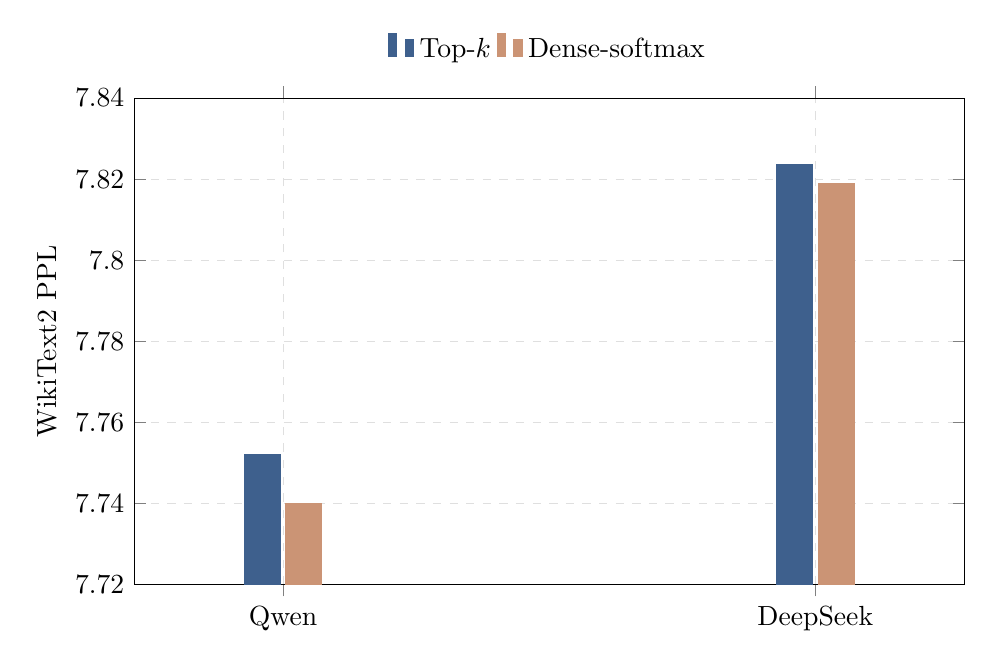
\begin{tikzpicture}
\begin{axis}[
    width=\columnwidth,
    height=0.64\columnwidth,
    ybar,
    bar width=13pt,
    ymin=7.72,
    ymax=7.84,
    ylabel={WikiText2 PPL},
    symbolic x coords={Qwen, DeepSeek},
    xtick=data,
    enlarge x limits=0.28,
    legend style={at={(0.5,1.05)}, anchor=south, legend columns=2, draw=none},
    grid=major,
    grid style={dashed,gray!25},
]
\addplot+[fill=paletteBlue, draw=paletteBlue] coordinates {(Qwen,7.7520) (DeepSeek,7.8237)};
\addplot+[fill=paletteTan, draw=paletteTan] coordinates {(Qwen,7.7399) (DeepSeek,7.8188)};
\legend{Top-$k$, Dense-softmax}
\end{axis}
\end{tikzpicture}
\caption{\small{Routing statistics 消融。两组实验均固定 routing power $p=2.0$ 且不启用 expert clustering；PPL 越低越好。}}
\label{fig:ablation_routing_statistics}
\end{figure}

\begin{figure}[htbp]
\centering
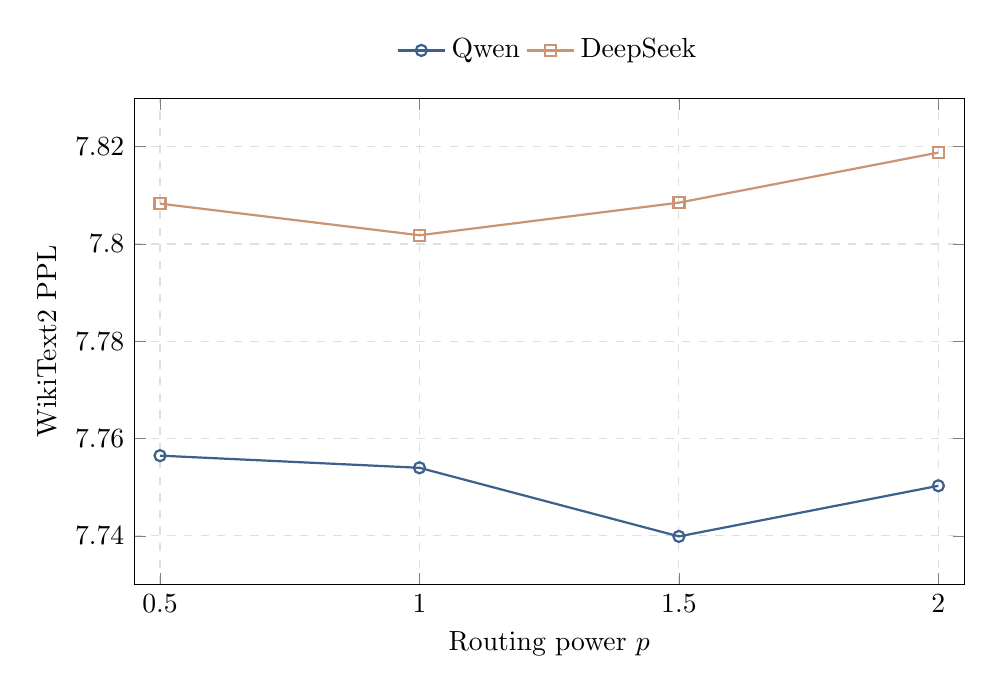
\begin{tikzpicture}
\begin{axis}[
    width=\columnwidth,
    height=0.64\columnwidth,
    xlabel={Routing power $p$},
    ylabel={WikiText2 PPL},
    xmin=0.45,
    xmax=2.05,
    ymin=7.73,
    ymax=7.83,
    xtick={0.5,1.0,1.5,2.0},
    legend style={at={(0.5,1.05)}, anchor=south, legend columns=2, draw=none},
    grid=major,
    grid style={dashed,gray!25},
]
\addplot+[paletteBlue, mark=o, thick] coordinates {(0.5,7.7565) (1.0,7.7540) (1.5,7.7399) (2.0,7.7503)};
\addplot+[paletteTan, mark=square, thick] coordinates {(0.5,7.8083) (1.0,7.8018) (1.5,7.8085) (2.0,7.8188)};
\legend{Qwen, DeepSeek}
\end{axis}
\end{tikzpicture}
\caption{\small{Routing power $p$ 消融。所有结果均使用 dense-softmax statistics，稀疏率为 $50\%$，不启用 expert clustering；PPL 越低越好。}}
\label{fig:ablation_routing_power}
\end{figure}

\begin{figure}[htbp]
\centering
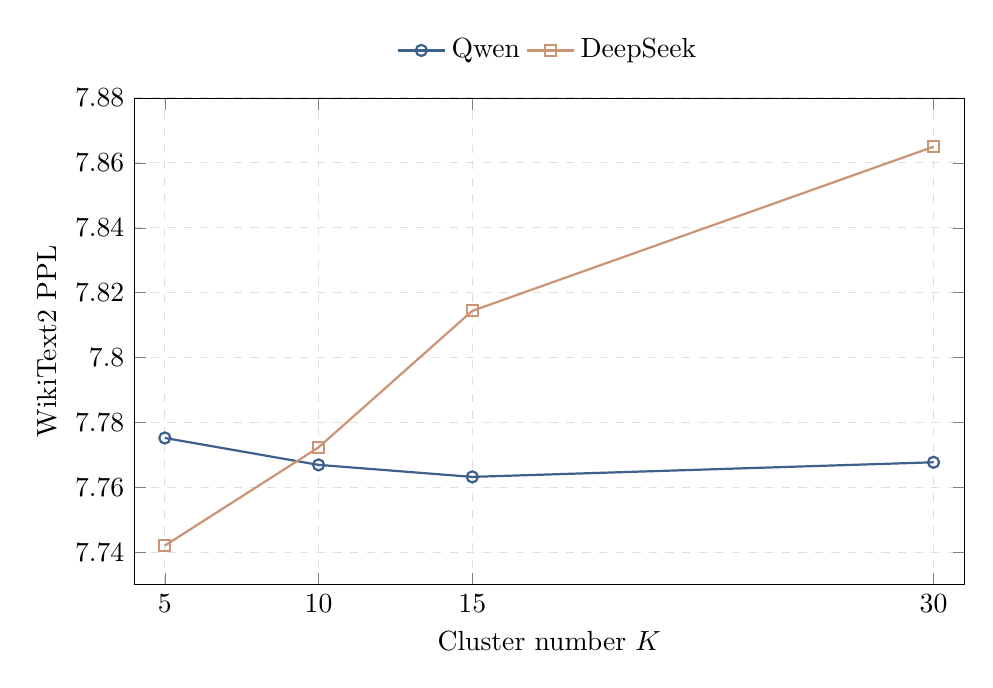
\begin{tikzpicture}
\begin{axis}[
    width=\columnwidth,
    height=0.64\columnwidth,
    xlabel={Cluster number $K$},
    ylabel={WikiText2 PPL},
    xmin=4,
    xmax=31,
    ymin=7.73,
    ymax=7.88,
    xtick={5,10,15,30},
    legend style={at={(0.5,1.05)}, anchor=south, legend columns=2, draw=none},
    grid=major,
    grid style={dashed,gray!25},
]
\addplot+[paletteBlue, mark=o, thick] coordinates {(5,7.7752) (10,7.7669) (15,7.7632) (30,7.7677)};
\addplot+[paletteTan, mark=square, thick] coordinates {(5,7.7420) (10,7.7723) (15,7.8144) (30,7.8650)};
\legend{Qwen, DeepSeek}
\end{axis}
\end{tikzpicture}
\caption{\small{Router-trace expert clustering 消融。所有结果均使用 dense-softmax statistics 与 $p=1.5$，稀疏率为 $50\%$；PPL 越低越好。}}
\label{fig:ablation_cluster_k}
\end{figure}


\subsection{Structured 2:4 GEMM Latency}

图 \ref{fig:moe_24_gemm_speedup} 报告了 MoE expert linear layers 在结构化 2:4 稀疏下的 GEMM speedup。
小 token batch 下 2:4 kernel 存在额外开销，但当 token 数增加后，2:4 稀疏 GEMM 开始体现加速收益。
\begin{figure}[htbp]
\centering
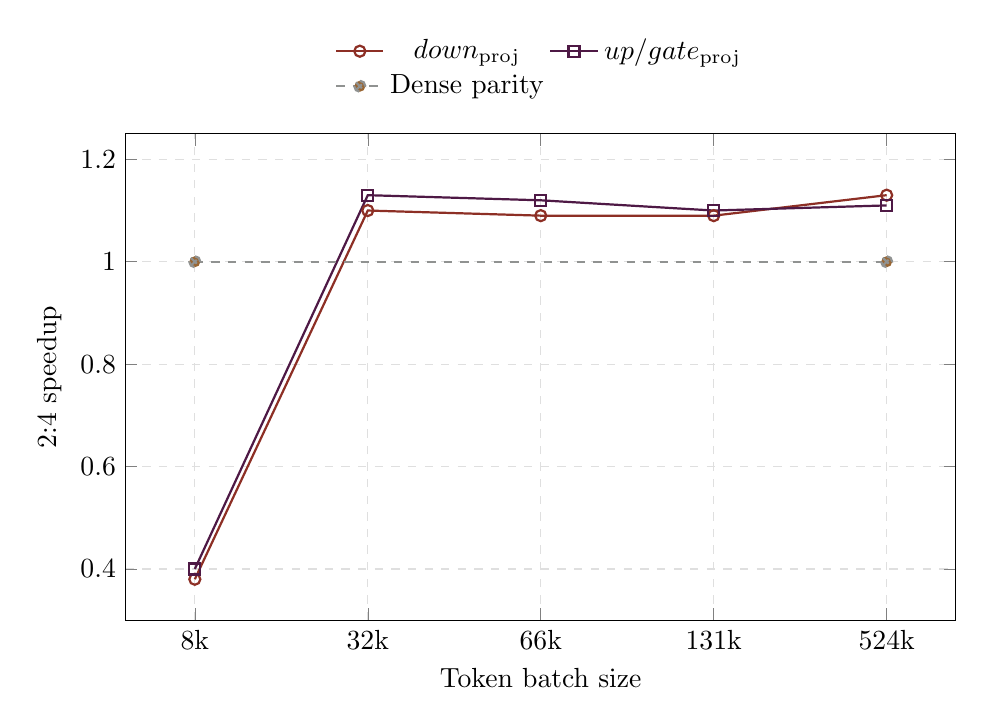
\begin{tikzpicture}
\begin{axis}[
    width=\columnwidth,
    height=0.64\columnwidth,
    xlabel={Token batch size},
    ylabel={2:4 speedup},
    symbolic x coords={8k,32k,66k,131k,524k},
    xtick=data,
    ymin=0.3,
    ymax=1.25,
    legend style={at={(0.5,1.05)}, anchor=south, legend columns=2, draw=none},
    grid=major,
    grid style={dashed,gray!25},
]
\addplot+[paletteRed, mark=o, thick] coordinates {(8k,0.38) (32k,1.10) (66k,1.09) (131k,1.09) (524k,1.13)};
\addplot+[palettePurple, mark=square, thick] coordinates {(8k,0.40) (32k,1.13) (66k,1.12) (131k,1.10) (524k,1.11)};
\addplot+[paletteGray, dashed, thick] coordinates {(8k,1.0) (524k,1.0)};
\legend{$down_{\mathrm{proj}}$, $up/gate_{\mathrm{proj}}$, Dense parity}
\end{axis}
\end{tikzpicture}
\caption{\small{MoE expert linear layers 在结构化 2:4 稀疏下的 GEMM speedup。原始 latency 单位为 milliseconds；speedup 高于 $1.0\times$ 表示 2:4 GEMM 快于 dense GEMM。在 $8$k tokens 时 2:4 GEMM 仍慢于 dense GEMM，speedup 约为 $0.38$--$0.40\times$；从 $32$k tokens 开始，down projection 与 up/gate projection 的 speedup 稳定在约 $1.09$--$1.13\times$。}}
\label{fig:moe_24_gemm_speedup}
\end{figure}


\section{Conclusion}

普通 Wanda 的成功来自一个简洁的局部线性扰动近似。
但 MoE-SwiGLU 模型引入了路由器、expert 分工、乘性门控和非线性调制，使得普通线性层近似在高稀疏率下变得不充分。
我们提出的 MoE-Wanda 从 MoE 层输出扰动出发，为 down/up/gate projection 分别构造路由感知剪枝分数，并通过 dense-softmax 统计、routing power 和 router-trace expert clustering 提升高稀疏率下的稳定性。
该方法的核心逻辑是将剪枝分数从“输入激活是否大”推进到“置零该权重会对 MoE 层输出造成多大路由加权扰动”。
这也是其相对普通 Wanda 的主要创新。

\begin{thebibliography}{99}

\bibitem{shazeer2017outrageously}
Noam Shazeer, Azalia Mirhoseini, Krzysztof Maziarz, Andy Davis, Quoc Le, Geoffrey Hinton, and Jeff Dean.
\newblock Outrageously Large Neural Networks: The Sparsely-Gated Mixture-of-Experts Layer.
\newblock In \emph{ICLR}, 2017.

\bibitem{lepikhin2020gshard}
Dmitry Lepikhin, HyoukJoong Lee, Yuanzhong Xu, Dehao Chen, Orhan Firat, Yanping Huang, Maxim Krikun, Noam Shazeer, and Zhifeng Chen.
\newblock GShard: Scaling Giant Models with Conditional Computation and Automatic Sharding.
\newblock In \emph{ICLR}, 2021.

\bibitem{fedus2021switch}
William Fedus, Barret Zoph, and Noam Shazeer.
\newblock Switch Transformers: Scaling to Trillion Parameter Models with Simple and Efficient Sparsity.
\newblock \emph{Journal of Machine Learning Research}, 23(120):1--39, 2022.

\bibitem{jiang2024mixtral}
Albert Q. Jiang et al.
\newblock Mixtral of Experts.
\newblock arXiv:2401.04088, 2024.

\bibitem{deepseekv2}
DeepSeek-AI et al.
\newblock DeepSeek-V2: A Strong, Economical, and Efficient Mixture-of-Experts Language Model.
\newblock arXiv:2405.04434, 2024.

\bibitem{frantar2023sparsegpt}
Elias Frantar and Dan Alistarh.
\newblock SparseGPT: Massive Language Models Can Be Accurately Pruned in One-Shot.
\newblock In \emph{ICML}, 2023.

\bibitem{sun2023wanda}
Mingjie Sun, Zhuang Liu, Anna Bair, and J. Zico Kolter.
\newblock A Simple and Effective Pruning Approach for Large Language Models.
\newblock arXiv:2306.11695, 2023.

\bibitem{moepruner2024}
Yanyue Xie, Zhi Zhang, Ding Zhou, Cong Xie, Ziang Song, Xin Liu, Yanzhi Wang, Xue Lin, and An Xu.
\newblock MoE-Pruner: Pruning Mixture-of-Experts Large Language Model using the Hints from Its Router.
\newblock arXiv:2410.12013, 2024.

\bibitem{zhang2025diversifying}
Zeliang Zhang, Xiaodong Liu, Hao Cheng, Chenliang Xu, and Jianfeng Gao.
\newblock Diversifying the Expert Knowledge for Task-Agnostic Pruning in Sparse Mixture-of-Experts.
\newblock arXiv:2407.09590, 2024.

\bibitem{guo2025cprune}
Hongcheng Guo et al.
\newblock Cluster-Driven Expert Pruning for Mixture-of-Experts Large Language Models.
\newblock arXiv:2504.07807, 2025.

\end{thebibliography}

\end{document}
